% id: 130-57
% book: 베이직쎈 대수 · 07 삼각함수의 그래프
% section: 개념 48 삼각부등식
% passage: 다음 부등식을 푸시오.
% figure: none
% answer: 
% answer_source: 
% variant_level: 0 (원본 전사)
% 이 파일은 build.mjs 가 items.json 에서 만든다. 고칠 때는 items.json 을 고친다.
\smash{\raisebox{4.5mm}{\dmkichul{베이직쎈 대수 130쪽 57번}}}
$\cos x\le-\dfrac{\sqrt{3}}{2}$ \dmcondfill{$0\le x<2\pi$}{}
\dmhint{주어진 부등식의 해는 함수 $y=\cos x\ (0\le x<2\pi)$의 그래프가 직선 $y=\blank$과 만나는 부분 또는 직선보다 아래쪽에 있는 부분의 $x$의 값의 범위이다.\par\smallskip\dispeq{% 130-57(130쪽) — 🎯 힌트 안 그래프: $y=\cos x$ $(0\le x<2\pi)$ 의 그래프와 직선 $y=-\frac{\sqrt{3}}{2}$.
% 스캔 화질이 낮아 TikZ 로 다시 그림. 라벨은 원문에 있는 것만 — $1$·$-1$, $\frac{\pi}{2}$·$\pi$·$\frac{3}{2}\pi$·$2\pi$.
% 원문처럼 직선보다 아래쪽에 있는 곡선 부분만 색을 넣었고, 그 양 끝 $x$좌표(= 답)는 원문에도 적혀 있지 않으므로 쓰지 않는다.
% $\frac{\pi}{2}$·$\frac{3}{2}\pi$ 는 곡선을 피해 원문처럼 아래쪽에 두고 가는 지시선으로 축의 자리를 가리킨다.
\begin{tikzpicture}[line width=0.6pt, x=0.80cm, y=0.72cm]
  \draw[dotted, line width=0.5pt] (0,1) -- (6.2832,1) (6.2832,0) -- (6.2832,1);
  \draw[dotted, line width=0.5pt] (0,-1) -- (4.7124,-1) (3.1416,0) -- (3.1416,-1);
  \draw[->, >=stealth, line width=0.7pt] (-0.65,0) -- (7.45,0) node[above=1pt, font=\footnotesize] {$x$};
  \draw[->, >=stealth, line width=0.7pt] (0,-1.90) -- (0,1.80) node[left=1pt, font=\footnotesize] {$y$};
  \draw[line width=0.6pt] (-0.65,-0.8660) -- (7.05,-0.8660);
  \draw[line width=0.7pt, domain=0:6.2832, samples=140, smooth] plot (\x, {cos(57.2958*\x)});
  \draw[red!75, line width=0.9pt, domain=2.6180:3.6652, samples=60, smooth] plot (\x, {cos(57.2958*\x)});
  \fill (0,1) circle (1.7pt);
  \draw[fill=white, line width=0.5pt] (6.2832,1) circle (1.7pt);
  \fill[red!75] (2.6180,-0.8660) circle (1.7pt);
  \fill[red!75] (3.6652,-0.8660) circle (1.7pt);
  \node[anchor=east, font=\footnotesize] at (-0.12,1) {$1$};
  \node[anchor=east, font=\footnotesize] at (-0.12,-1) {$-1$};
  \node[anchor=north east, font=\footnotesize] at (-0.04,-0.06) {$\pt{O}$};
  \node[anchor=south, font=\footnotesize, fill=white, inner sep=0.6pt] at (3.1416,0.05) {$\pi$};
  \node[anchor=north, font=\footnotesize] at (1.24,-1.30) {$\dfrac{\pi}{2}$};
  \draw[line width=0.4pt] (1.5708,-0.08) to[out=250, in=60] (1.30,-1.28);
  \node[anchor=north, font=\footnotesize] at (5.05,-1.30) {$\dfrac{3}{2}\pi$};
  \draw[line width=0.4pt] (4.7124,-0.08) to[out=290, in=120] (4.99,-1.28);
  \node[anchor=north, font=\footnotesize] at (6.2832,-0.10) {$2\pi$};
  \node[anchor=south east, font=\footnotesize] at (6.15,1.04) {$y=\cos x$};
  \node[anchor=west, font=\footnotesize] at (7.10,-0.8660) {$y=-\dfrac{\sqrt{3}}{2}$};
\end{tikzpicture}
}\par\smallskip\noindent 따라서 구하는 해는 \quad $\blank\le x\le\blank$}
